%        File: arfc-beamer.tex
%     Created: Sun May 5 10:00 PM 2013 C
%


%\documentclass[11pt,handout]{beamer}
\documentclass[9pt]{beamer}
\usetheme[white]{Illinois}
%\title[short title]{long title}
\title[Fuel processing simulation tool for liquid-fueled reactors]{Fuel 
processing simulation tool for liquid-fueled nuclear reactors}
%\subtitle[short subtitle]{long subtitle}
%\subtitle[Short SubTitle]{Mostly Kittens}
%\author[short name]{long name}
\author[Andrei Rykhlevskii]{Andrei Rykhlevskii}
%\date[short date]{long date}
\date[07.01.2020]{July 1, 2020}
%\institution[short name]{long name}
\institute[UIUC]{University of Illinois at Urbana-Champaign}

%\usepackage{enumitem}
\usepackage{lmodern}
\usepackage{verbatim}
\usepackage{tikz}
\usepackage{amsfonts}
\usepackage{amsmath}
\usepackage{array}
\usepackage{caption}  % allows center figures caption
\usepackage{xspace}
\usepackage{notoccite}
\usepackage{graphicx}
\usepackage{animate}
\usepackage{subfigure}
\usepackage{booktabs} % nice rules for tables
\usepackage{microtype} % if using PDF
\usepackage{bigints}
\usepackage[absolute,overlay]{textpos}
%\usepackage{minted}
\usepackage{xcolor}
\usepackage{soul}
\newcommand{\hlc}[2][yellow]{{%
    \colorlet{foo}{#1}%
    \sethlcolor{foo}\hl{#2}}%
}
\newcommand{\units}[1] {\:\text{#1}}%
\newcommand{\SN}{S$_N$}%{S$_\text{N}$}%{$S_N$}%
\DeclareMathOperator{\erf}{erf}
%I need some complimentary error funcitons... 
\DeclareMathOperator{\erfc}{erfc}
% Total slides number manual
%\def\inserttotalframenumber{51}
%%--------------------------------%%
%page numbers
\setbeamertemplate{page number in head/foot}[appendixframenumber]
\setbeamertemplate{caption}[numbered]
%Those icons in the references are terrible looking
\setbeamertemplate{bibliography item}[text]
\setbeamercovered{dynamic}
%%%% Acronym support

\usepackage[acronym,toc]{glossaries}
\include{acros}

\makeglossaries

%try to get rid of header on title page\dots
\makeatletter
    \newenvironment{withoutheadline}{
        \setbeamertemplate{headline}[default]
        \def\beamer@entrycode{\vspace*{-\headheight}}
    }{}
\makeatother

\begin{document}
%%%%%%%%%%%%%%%%%%%%%%%%%%%%%%%%%%%%%%%%%%%%%%%%%%%%%%%%%%%%%
%% From uw-beamer Here's a handy bit of code to place at 
%% the beginning of your presentation (after \begin{document}):
\newcommand*{\alphabet}{ABCDEFGHIJKLMNOPQRSTUVWXYZabcdefghijklmnopqrstuvwxyz}
\newlength{\highlightheight}
\newlength{\highlightdepth}
\newlength{\highlightmargin}
\setlength{\highlightmargin}{2pt}
\settoheight{\highlightheight}{\alphabet}
\settodepth{\highlightdepth}{\alphabet}
\addtolength{\highlightheight}{\highlightmargin}
\addtolength{\highlightdepth}{\highlightmargin}
\addtolength{\highlightheight}{\highlightdepth}
\newcommand*{\Highlight}{\rlap{\textcolor{HighlightBackground}{\rule[-\highlightdepth]{\linewidth}{\highlightheight}}}}
%%%%%%%%%%%%%%%%%%%%%%%%%%%%%%%%%%%%%%%%%%%%%%%%%%%%%%%%%%%%%

\begin{withoutheadline}
\frame{
  \titlepage
}
\end{withoutheadline}

%%--------------------------------%%
\AtBeginSection[]{
\begin{frame}
  \frametitle{Outline}
  \tableofcontents[currentsection]
\end{frame}
}

\section{Introduction}
\subsection{\glspl{MSR}}

\begin{frame}
\frametitle{MSR (Molten Salt Reactor) types}
\begin{textblock*}{12cm}(0.4cm,2.1cm) % {block width} (coords)
	\begin{overlayarea}{\linewidth}{20\baselineskip}
		\begin{block}{Stationary Fuel}<1-4>
			\begin{enumerate}
				\item \textbf{Solid}
				\begin{itemize}
					\item Graphite block with TRISO fuel, clean salt works as 
					coolant (Fluoride-Salt-Cooled High-Temperature Reactor 
					(FHR))
					\item Plate Fuel: hexagonal fuel assembly is similar in 
					shape 
					to a typical sodium-cooled reactor
					\item Fuel Inside Radial Moderator (FIRM)
				\end{itemize}
			\end{enumerate}
		\end{block}
		
		\begin{block}{Mobile Fuel}<2-4>
			\begin{enumerate}
				\item \textbf{Solid}
				\begin{itemize}
					\item<2-> Mobile solid fuel elements (pebbles) cooled by 
					clean salt (PB-FHR by Kairos Power)
				\end{itemize}
				\item<3-> \textbf{Liquid}
				\begin{itemize}
					\item<3-> Without on-site fuel reprocessing facility 
					(TerraPower \glsfirst{MCFR})
					\item<4-> \textbf{With on-site fuel reprocessing} 
					(\glsfirst{TAP} MSR, \glsfirst{MSBR})
				\end{itemize}
			\end{enumerate}
		\end{block}
	\end{overlayarea}
\end{textblock*}
\end{frame}

\begin{frame} % Add another slide with red rectangular around reprocessing 
%system
\frametitle{Circulating-fuel reactor with on-site reprocessing system}
% Weinberg 1945, U sulfate in water, 140kW
\vspace{-2mm}
\begin{figure}[t]
		\begin{overprint}
			\onslide<1>\includegraphics[height=0.6\textwidth]{./images/msbr_scheme.png}
			\onslide<2>\includegraphics[height=0.6\textwidth]{./images/msbr_scheme_box.png}
		\end{overprint}
	\caption{The MSBR is an example of reactor design with 
	\textbf{liquid, mobile, circulating} fluoride salt fuel 
	(reproduced from Rosenthal \emph{et al.} 
	\cite{rosenthal_molten-salt_1970}).}
\end{figure}   

\end{frame}

\begin{frame}
\frametitle{Why Molten Salt Reactors with circulating fuel?}
\begin{block}{Liquid-fueled \gls{MSR} designs have following \textbf{potential} advantages:}
	\begin{enumerate}
		\itemsep1em
		\item High coolant temperature (600-750$^{\circ}$C) 
		$\Rightarrow$ potentially high thermal efficiency, process 
		heat for chemical industry or hydrogen production
		\item Fuel diversity ($^{235}$U, $^{233}$U, Thorium, U/Pu)
		\item Strong negative fuel temperature feedback 
		\item Passive safety $\Rightarrow$ fuel drains into tanks 
		in emergency
		\item High fuel utilization $\Rightarrow$ reduced spent fuel 
		generation
		\item<2> \textbf{On-line (continuous) fuel reprocessing and refueling}
	\end{enumerate}
\end{block}

\end{frame}


\subsection{Background}

\begin{frame}
\frametitle{On-line fuel processing and on-line refueling pros and 
cons}
\begin{block}{Advantages}
	\begin{enumerate}
		\item Neutron economy
		\item Fuel utilization
		\item Refueling without outages
		\item Reduced excess reactivity
	\end{enumerate}
\end{block}

\begin{block}{Disadvantages}
	\begin{enumerate}
		\item Chemical separation is challenging
		\item Fuel salt balance in the primary loop complicates operation
		\item \textbf{Existing burnup calculation software cannot model it}
	\end{enumerate}
\end{block}

\end{frame}


\begin{frame}
\frametitle{Fuel salt burnup and reprocessing}
		\vspace{-5mm}
	\begin{figure}[t]
		\hspace*{-0.2in}
			\includegraphics[height=0.6\textwidth]{./images/periodic_map.png}
		\vspace{-0.15in}
		\caption{Processing options for MSR fuels (figure reproduced from Ahmed \emph{et al.}  \cite{ahmad_neutronics_2015}).}
	\end{figure}               
\end{frame}

\begin{comment}
\begin{frame}
\frametitle{On-line fuel salt reprocessing system functions}
\begin{block}{Removing poisonous fission products}
	\begin{itemize}
		\item Noble gas (e.g., centrifugal gas separator)
		\item Noble metal (e.g., large filter with nickel fibers)
       \item Rare earth (separation based on different chemical potentials)
		%\item Ideally, remove 100\% of target element but realistically, 
		%30-90\%
		\item Some valuable rare metals (Rh,Pd) may be recovered %%Rh - $5000, 
%%%Pd - $1500, Pl - $900, Ir - $1480
	\end{itemize}
\end{block}

\begin{block}{Injecting fresh fuel}
	\begin{itemize}
		\item Fissile material ($^{233}$U, $^{235}$U, $^{239}$Pu)
		\item Fertile material ($^{232}$Th, $^{238}$U)
		\item Maintain fuel salt inventory in the primary loop
		\item Maintain reactor criticality (ideally, $k_{eff}=1.0$)
	\end{itemize}
\end{block}

\end{frame}
\end{comment}

\begin{frame}
\frametitle{Continuous vs batch-wise fuel processing  and refueling (1/3)}
\vspace{-8mm}
\begin{block}{Classic Bateman equation}
	%Core material is circulated to or from the core at specific intervals:
	\begin{align}
	\frac{dN_i}{dt} &= \sum_{m=1}^{M}l_{im}\lambda_mN_m + 
	\phi\sum_{m=1}^{M}f_{im}\sigma_mN_m - (\lambda_i + \phi\sigma_i)N_i + 
	F_i\Big|\quad{i\in [1,M]} \nonumber\\
	N_i &= \mbox{atom density of nuclide i} \nonumber \\
	M &= \mbox{number of nuclides} \nonumber \\
	l_{im} &= \mbox{fraction of decays of nuclide m that result in formation 
	of 
		nuclide i}\nonumber \\
	\lambda_i &= \mbox{radioactive decay constant of nuclide i} \nonumber \\
	\phi &= \mbox{neutron flux, averaged over position and energy} \nonumber \\
	f_{im} &= \mbox{fraction of neutron absorption by nuclide m leading to the 
		formation of nuclide i} \nonumber \\
	\sigma_m &= \mbox{average neutron absorption cross section of nuclide m} 
	\nonumber \\
	F_i &= \mbox{production rate of nuclide i directly from fission}\nonumber
	\end{align}
\end{block}
\end{frame}

\begin{frame}
\frametitle{Continuous vs batch-wise fuel processing  and refueling (2/3)}
\vspace{-1.3mm}
\begin{block}{Bateman equation with continuous removals and feed}
	\begin{align}
	\frac{dN_i}{dt} &= \sum_{m=1}^{M}l_{im}\lambda_mN_m + 
	\phi\sum_{m=1}^{M}f_{im}\sigma_mN_m - (\lambda_i + \phi\sigma_i + 
	\textcolor{red}{r_i - 
		f_i})N_i + F_i\Big|\quad{i\in [1,M]} \nonumber \\
	N_i &= \mbox{atom density of nuclide i} \nonumber \\
	M &= \mbox{number of nuclides} \nonumber \\
	l_{im} &= \mbox{fraction of decays of nuclide m that result in formation 
	of 
		nuclide i}\nonumber \\
	\lambda_i &= \mbox{radioactive decay constant of nuclide i} \nonumber \\
	\phi &= \mbox{neutron flux, averaged over position and energy} \nonumber \\
	f_{im} &= \mbox{fraction of neutron absorption by nuclide m leading to the 
		formation of nuclide i} \nonumber \\
	\sigma_m &= \mbox{average neutron absorption cross section of nuclide m} 
	\nonumber \\
	\textcolor{red}{r_i} & \mkern4mu \textcolor{red}{=} \mbox{\space 
	\textcolor{red}{continuous removal rate of nuclide i from the system}} 
	\nonumber \\
	\textcolor{red}{f_i} & \mkern4mu  \textcolor{red}{=} \mbox{\space 
	\textcolor{red}{continuous feed rate of nuclide i}} \nonumber \\
	F_i &= \mbox{production rate of nuclide i directly from fission}\nonumber
	\end{align}
\end{block}
\end{frame}


\begin{frame}
\frametitle{Continuous vs batch-wise fuel processing and refueling (3/3)}
\begin{block}{Batch-wise approach}
	Core material is circulated to or from the core at specific 
	intervals		
\end{block}
\begin{figure}[t]
	\hspace{3mm}
	\includegraphics[height=0.4\textwidth]{./images/batch-wise.png}
	\caption{Typical flowchart for batch-wise reprocessing and refueling 
		\cite{li_optimization_2018}.}
\end{figure}               
\end{frame}


\begin{frame}
\frametitle{Fuel salt reprocessing simulation approaches pros and cons}

\begin{enumerate}
	\itemsep2em
	\item Continuous: removal and feed terms are added to the Bateman equation
	\begin{itemize}
		\itemsep1em
		\item[$\mathbf{+}$] allows coarse burnup timesteps
		\item[$\mathbf{-}$] requires a sophisticated algorithm for rebalancing 
		the salt mass 
	\end{itemize}
	\item \textbf{Batch-wise}: burnup simulation stops and restarts with 
	modified fuel composition
	\begin{itemize}
		\itemsep1em
		\item[$\mathbf{+}$] composition calculation models removals and feeds 
		at each stop/start
		\item[$\mathbf{+}$] easy to balance the salt mass in the primary loop
		\item[$\mathbf{-}$] requires very fine burnup timesteps
	\end{itemize}
\end{enumerate}
\end{frame}


\begin{frame}
\frametitle{Published work in on-line reprocessing and modeling}

  \begin{textblock*}{12.5cm}(0.1cm,1.6cm) % {block width} (coords)
	\begin{table}[t]
	\fontsize{7}{9}\selectfont
	\caption{Tools and methods for liquid-fueled \gls{MSR} fuel depletion 
	analysis.}
			\vspace{-2mm}
	\begin{tabularx}{\textwidth}{p{2.5cm} X X X p{3cm}} 
		\hline 
		&Nuttin \emph{et al.}, 2005 \cite{nuttin_potential_2005}& Aufiero \emph{et al.}, 
		2013 \cite{aufiero_extended_2013} & Betzler \emph{et al.}, 2018 
		\cite{betzler_fuel_2018}&Proposed work \\ 
		\hline
		Neutronics & \gls{MCNP} & Serpent 2 & SCALE6.2 & Serpent 2 \\
		software   & REM &           & ORIGEN-S &  \\
	               & stochastic & stochastic & deterministic & stochastic\\ [3pt]
		Geometry  & unit cell & full-core 3D & unit cell & full-core 3D\\ [3pt]
		Removal/feed  & continuous &continuous & batch-wise & batch-wise\\ [3pt]
        Separation efficiency & fixed & fixed & fixed & \textcolor{red}{function of many parameters} \\[3pt]
        Fuel reprocessing plant & ``black box'' & ``black box'' & ``black box'' & \textcolor{red}{realistic multi-component model} \\[3pt]
        Reactivity control & continuous& continuous & batch feed & 
        \textcolor{red}{periodic adjustment of geometry and fissile material 
        injection}\\[3pt]
        Power level & \multicolumn{3}{c}{fixed}& \textcolor{red}{variable} 
        \\[3pt]
		Thermal feedback & Doppler only & Not considered & Doppler only & 
		Doppler$+$\textcolor{red}{density+thermal expansion}\\[3pt]
		Void coefficient  & \multicolumn{3}{c}{Not considered} & 
		\textcolor{red}{For BOL and EOL} \\[3pt]
		Control rod worth & \multicolumn{3}{c}{Not considered} & 
		\textcolor{red}{Total} \\[3pt]
		\hline
	\end{tabularx}
	\label{tab:msr_codes}
\end{table}
\end{textblock*}

\end{frame}


\begin{frame}
\frametitle{Technical gap in the state of the art}
\vspace{-0.2in}
\begin{block}{Static ``black'' box assumptions in the literature}
	\begin{equation*}
	{\tiny  
		\setlength{\abovedisplayskip}{6pt}
		\setlength{\belowdisplayskip}{\abovedisplayskip}
		\setlength{\abovedisplayshortskip}{0pt}
		\setlength{\belowdisplayshortskip}{3pt}
	\begin{aligned}
	\begin{bmatrix}
	N^{in}_{0} \\ \vdots \\ N^{in}_{e} \\ \vdots \\ N^{in}_{E} \\
	\end{bmatrix} 
	\times
	\begin{bmatrix}
	\epsilon_{0} \\ \vdots \\ \epsilon_{e} \\ \vdots \\ \epsilon_{E} \\
	\end{bmatrix} =
	\begin{bmatrix}
	N^{out}_{0}\\ \vdots \\ N^{out}_{e} \\ \vdots \\N^{out}_{E}  \\
	\end{bmatrix}
	\end{aligned}
	}
	\end{equation*}
	\begin{itemize}
		\item \textbf{Assume time-independent separation efficiency ($\epsilon_e$).} Realistically, 
		it is \textbf{time-dependent}.
		\item \textbf{Assume $\epsilon_e$ is independent of the reactor operational 
		parameters.} But $\epsilon_e$ depends on \textbf{temperature, power level, current fuel salt isotopic composition, and material flow rate}.
		\item \textbf{Processing plant is lumped in a single ``black	box'' component.} But the system contains many components connected in series, parallel, or both. 
	\end{itemize}
\end{block}
\end{frame}

\subsection{Research objectives}

\begin{frame}
  \frametitle{Research objectives}
                  \vspace*{-0.05in}
      The main objective of the current work is to develop the on-line  
      reprocessing simulation package, SaltProc, for liquid-fueled reactors 
      depletion simulations.
     \begin{block}{SaltProc desired capabilities:}<1-4>
         \begin{enumerate}
         		%\itemsep1em
                \item \textbf{Open-source} with continuous tests and 
				automatic documentation system 
                \item \textbf{Realistic} multi-component fuel 
                reprocessing system modeling
                \item Reactivity control by \textbf{changing geometry} of 
                the core during simulation
                \item \textbf{Variable} extraction efficiency support defined 
                as function of many parameters
         \end{enumerate}
      \end{block}
            \vspace{-0.1in}
	\begin{block}{SaltProc demonstration and validation for TAP MSR and 
	MSBR}<2-4>
		\begin{enumerate}
			\item<2-4> \textbf{Lifetime-long} depletion with ideal/realistic 
			$\epsilon_e$
			\item<3-4> Short-term depletion \textbf{during load-following 
			transient}
			\item<4> Safety parameters ($\alpha_{T}, \alpha_{V}$, control rod 
			worth) \textbf{evolution during long- and short-term operation}
		\end{enumerate}
	\end{block}
\end{frame}

\section{Methodology}
\subsection{Fuel salt reprocessing system}

\begin{frame}
  \frametitle{Fuel salt reprocessing system overview: gas separation}
  Gaseous fission products (e.g., Xe, Kr) must be removed from the fuel salt 
  to avoid reactor poisoning ($\Sigma_{a,^{135}Xe}=10^6\dots10^7$b). 
  
      \begin{columns}
      	\column[t]{4.0cm}
    \begin{block}{Noble gas removal}
      \begin{enumerate}
      	\item[\textcolor{blue}{\textbullet}] bubble generator injects He 
      	bubbles in the salt stream
      	\item[\textcolor{green}{\textbullet}] noble gas migrate to the He 
      	bubbles 
      	\item[\textcolor{red}{\textbullet}] gas separator discharges the 
      	poison-rich bubbles
      \end{enumerate}
    \end{block}    	
      	
     	\column[t]{8cm}
  \begin{figure}[t]
	  \centering
	  		\vspace{-1mm}
		\includegraphics[width=\textwidth]{./images/msbr_gas_separation.pdf}
	\caption{Schematic flow diagram of the \gls{MSBR} gas separation system 
	(figure reproduced from Robertson \emph{et al.}  
	\cite{robertson_conceptual_1971}).} 
    \end{figure}

	\end{columns}
\end{frame}

\begin{frame}
  \frametitle{Mathematical model for gas separation efficiency}
  		\vspace{-1mm}
Xenon removal efficiency ($\epsilon_{Xe}$) in a gas separation system is 
\cite{peebles_removal_1968, sada_gas-liquid_1987}:
\begin{align}
& \qquad\qquad \epsilon_{Xe} = \frac{1-e^{-\beta}}{1+\alpha} \nonumber \\
\alpha &= \frac{RTQ_{L}}{HQ_{G}} \nonumber \\
\beta &= K_L \frac{6}{d_b} \frac{Q_G}{Q_G+G_L} \frac{A_C L (1+\alpha)}{Q_{L}} 
\nonumber \\
Q_{L}&= \mbox{volumetric salt flow rate [$m^3/s$]} \nonumber \\
Q_{G}&= \mbox{volumetric helium flow rate [$m^3/s$]} \nonumber \\
H &= \mbox{Henry's law constant [$Pa\cdot mol^{-1}\cdot L$]} \nonumber \\
d_b &= \mbox{helium bubble diameter [m]} \nonumber \\
K_L &= \mbox{liquid phase mass transfer coefficient [m/s].} \nonumber
\end{align}
		\vspace{-6mm}
  \begin{figure}[t]
	\includegraphics[width=0.66\textwidth]{./images/pipeline_contactor.png}
	\vspace{-3mm}
	\caption{Flow diagram for gas separator (figure reproduced from Peebles 
		\emph{et al.} \cite{peebles_removal_1968}).}
\end{figure}

\end{frame}


%\begin{frame}
%\frametitle{Fuel processing system overview: rare earths and Pa removal}
%		\vspace{-2mm}
%	\begin{figure}[htp!] % replace 't' with 'b' to 
%		\centering
%			\includegraphics[width=0.57\textwidth]{../figures/flowsheet.pdf}
%			\vspace{-2mm}
%		\caption{Liquid metal (Bi) extraction system for the \gls{MSBR} 
%		(reproduced from Sorensen \cite{sorensen_one-fluid_2006}).} 
%	\end{figure}
%\end{frame}


\begin{frame}
\frametitle{Fuel processing system overview: TAP concept}
	\vspace{-2mm}
\begin{figure}[htp!] % replace 't' with 'b' to 
	\centering
	\includegraphics[width=0.75\textwidth]{../dissertation/figures/ch4/tap_primary_loop.png}
		\vspace{-2mm}
	\caption{Simplified \gls{TAP} primary loop design including off-gas system 
		(blue), nickel filter (orange) and liquid metal extraction system 
		(green) \cite{transatomic_power_transatomic_2019}.}
\end{figure}

\end{frame}

\begin{frame}
\frametitle{SaltProc demonstration for TAP concept input data}
\begin{textblock*}{12.5cm}(0.5cm,1.6cm) % {block width} (coords)
	%%%%%%%%%%%%%%%%%%%%%%%%%%%%%%%%%%%%%%%%
	\begin{table}[htbp!]
		\fontsize{6}{9}\selectfont
		\centering
		\caption{The effective cycle times and rates for fission products 
		removal \cite{robertson_conceptual_1971, betzler_implementation_2017}.}
			\vspace{-2mm}
		\begin{tabular}{p{0.14\textwidth} p{0.3\textwidth} p{0.11\textwidth} 
				p{0.11\textwidth}}
			\hline 
			\textbf{Processing group} & \qquad\qquad\qquad \textbf{Nuclides} & 
			\textbf{Removal Rate (s$^{-1}$)} & \textbf{Cycle time (at full 
			power)} 
			\\ \hline 
			\multicolumn{3}{c}{\textit{Elements removed in \gls{MSBR} and 
			adopted for the \gls{TAP}} 
					\cite{robertson_conceptual_1971}} \\
			Noble gases & Xe, Kr								  & 5.00E-2 & 
			20 
			sec \\
			Noble metals & Se, Nb, Mo, Tc, Ru, Rh, Pd, Ag, Sb, Te & 5.00E-2 & 
			20 
			sec \\
			Seminoble metals & Zr, Cd, In, Sn	  				  & 5.79E-8 & 
			200 
			days\\
			Volatile fluorides & Br, I 							  & 1.93E-7 & 
			60 
			days\\
			Rare earths & Y, La, Ce, Pr, Nd, Pm, Sm, Gd           & 2.31E-7 & 
			50 
			days\\
			\qquad & Eu & 2.32E-8 & 500 days \\
			Discard & Rb, Sr, Cs, Ba & 3.37E-9 & 3435 days \\
			\hline
			\multicolumn{3}{c}{\textit{Additional elements removed in 
			\gls{TAP}} 
				\cite{betzler_implementation_2017, 
					transatomic_power_corporation_neutronics_2016}} \\
			Noble gases & H								  	& 5.00E-2 & 20 
			sec    \\
			Noble metals & Ti, V, Cr, Cu						& 3.37E-9 & 
			3435 
			days \\
			Seminoble metals & Mn, Fe, Co, Ni, Zn, Ga, Ge, As   & 3.37E-9 & 
			3435 
			days \\
			Rare earths & Sc									& 3.37E-9 & 
			3435 
			days \\
			Discard & Ca										& 3.37E-9 & 
			3435 
			days \\
			\hline
			\multicolumn{3}{c}{\textit{Additional elements removed in 
			\gls{MSBR}} 
				\cite{robertson_conceptual_1971}} \\
			Protactinium & Pa  	& 3.86E-6 & 3 days    \\
			\hline
		\end{tabular}
		\label{tab:reprocessing_list}
	\end{table}
	\begin{itemize}
		\item Noble gas removal efficiency: variable, defined using 
		mathematical model
		\item Other FP removal efficiency: fixed and based on 
		Table~\ref{tab:reprocessing_list}
	\end{itemize}
\end{textblock*}
\end{frame}


\subsection{SaltProc tool design}


\begin{frame}
\frametitle{SaltProc class architecture}
	\begin{itemize}
		\item \textit{Simulation} class
			\begin{itemize}
				\item Manages simulation process
				\item Stores data into the HDF5 database
				\item Tracks time, power level
			\end{itemize}
		\item \textit{Depcode} class
			\begin{itemize}
				\item Contains attributes and methods for reading user's input
				\item Creates input files for depletion code
				\item Parses depletion code output 
			\end{itemize}
		\item \textit{Process} class
			\begin{itemize}
				\item Represents fuel processing system component
				\item Contains attributes of the component ($\vec{\epsilon}$, 
				throughput rate)
				\item Tracks waste stream
			\end{itemize}
		\item \textit{MaterialFlow} class
			\begin{itemize}
				\item Instances of that class represents the material flowing between processes
			\end{itemize}
	\end{itemize}
		\vspace{1mm}
	\begin{figure}[ht!] % replace 't' with 'b' to 
		\centering
		\begin{overprint}
		\onslide<1>\centerline{\includegraphics[width=0.6\textwidth]{../dissertation/figures/ch2/materialflow.pdf}}
		\onslide<2>\centerline{\includegraphics[width=0.6\textwidth]{../dissertation/figures/ch2/tap_materialflow.pdf}}
		\end{overprint}
		\vspace{-2mm}
		\caption{Schematic for passing material data between fuel processing 
		system components.}
	\end{figure}

\end{frame}


\begin{frame}
\frametitle{SaltProc flowchart}
\vspace{-4mm}
\begin{figure}[ht!] % replace 't' with 'b' to \centering
	\centering
	\includegraphics[width=1.08\textwidth]{../dissertation/figures/ch2/saltproc_flowchart.pdf}
		\vspace{-4mm}
	\caption{SaltProc v1.0 Python package flowchart.}
\end{figure}

\end{frame}


\begin{frame}
\frametitle{Multi-component fuel reprocessing system model in SaltProc}       

\begin{figure}[htp!] % replace 't' with 'b' to 
	\centering
	\vspace{-2mm}
	\begin{overprint}
	\onslide<1>\includegraphics[height=0.85\textheight]{./images/tap_saltproc_var_eps.png}
		\vspace{-2mm}
    \caption{\textcolor{green}{\gls{TAP}} reprocessing scheme for 
	SaltProc demonstration.}
	\onslide<2>\includegraphics[height=0.85\textheight]{./images/msbr_saltproc_var_eps.png}
		\vspace{-2mm}
	\caption{\textcolor{red}{\gls{MSBR}} reprocessing scheme for 
	SaltProc demonstration.}
	\end{overprint}
\end{figure}

\end{frame}


\begin{frame}[fragile]
\frametitle{DOT code used to describe TAP reprocessing system}
\small
\begin{verbatim}
digraph fuel {
==============================================================================
core_outlet -> sparger [label="100%", fontsize=20]
sparger -> waste_sparger [label="60% of\nXe, Kr, H", fontsize=20]
sparger -> entrainment_separator [label="100%", fontsize=20]
entrainment_separator -> nickel_filter [label="100%", fontsize=20]
entrainment_separator -> waste_entrainment_separator [label="97% of\nXe, Kr, 
%H", fontsize=20]
nickel_filter -> bypass [label="90%", fontsize=20]
bypass -> heat_exchanger [label="90%", fontsize=20]
nickel_filter -> waste_nickel_filter [label="100% of noble metals", 
%fontsize=20]
nickel_filter -> liquid_metal [label="10%", fontsize=20]
liquid_metal -> heat_exchanger [label="10%", fontsize=20]
liquid_metal -> waste_liquid_metal [label="57% of seminoble metals \n& RE", 
%fontsize=20]
heat_exchanger -> core_inlet [label="100%", fontsize=20]
LEU_feed -> core_inlet
==============================================================================
# Optional parameters to prettify plots
\end{verbatim}
\end{frame}
\section{Results}
\subsection{Lifetime-long depletion: MSBR}


\begin{frame}
\frametitle{Molten Salt Breeder Reactor (MSBR) design}

\begin{textblock*}{12.5cm}(0.1cm,2.1cm) % {block width} (coords)
	
	\begin{columns}
		\column[t]{6cm}
		%%%%%%%%%%%%%%%%%%%%%%%%%%%%%%%%%%%%%%%%
		\begin{table}[h!]
			\fontsize{7}{9}\selectfont
			\caption{Summary of principal data for the \gls{MSBR} 
				\cite{robertson_conceptual_1971}. }
			\vspace{-2mm}
			\begin{tabularx}{\textwidth}{ p{3.6cm}  X}
				\hline
				Thermal power				           		& 2250 MW$_{th}$\\ 
				Electric power		                		& 1000 MW$_e$   
				\\  
				Net thermal efficiency        			    & 44.4\%       	
				\\  
				Salt volume fraction in Zone I				& 0.132			\\ 
				Salt volume fraction in Zone II  			& 0.37			\\ 
				Fuel salt inventory (Zone I)				& 8.2 m$^3$     \\
				Fuel salt inventory (Zone II)				& 10.8 m$^3$    \\
				Fuel salt inventory (annulus)				& 3.8 m$^3$     \\
				Fuel salt components    & LiF-BeF$_2$-ThF$_4$-\newline
				$^{233}$UF$_4$\\  
				Fuel salt composition           & 71.75-16-\newline 12-	
				0.25mole\%	\\  
				Neutron spectrum						    & thermal \\
				\hline
			\end{tabularx}
		\end{table}
		%%%%%%%%%%%%%%%%%%%%%%%%%%%%%%%%%%%%%%%%%%%%%%%%
		
		\column[t]{5.6cm}
		\vspace{-1mm}
		\begin{figure}      
			\hspace{-12mm}
			\includegraphics[height=1.05\textwidth]{./images/plan_view_vessel.png}
			\caption{Plan view of \gls{MSBR} vessel 
				\cite{robertson_conceptual_1971}.}
		\end{figure}
	\end{columns}
	
\end{textblock*}

\end{frame}


\begin{frame}
\frametitle{Geometry of MSBR model (Serpent)}

\begin{textblock*}{12.5cm}(0.1cm,1.9cm) % {block width} (coords)
\begin{figure}      
	\includegraphics[width=\textwidth]{./images/geometry_main_views.png}
	\caption{An $XY$ (left) and $XZ$ (right) sections of \gls{MSBR} model. 
		The violet color represents graphite, the yellow - fuel salt 	
		\cite{rykhlevskii_full-core_2017}.}
\end{figure}
\end{textblock*}
\end{frame}

\begin{frame}
\frametitle{Moderator element geometry (Zone I)}
\begin{textblock*}{12.5cm}(0.1cm,1.9cm) % {block width} (coords)
\begin{figure}[t]
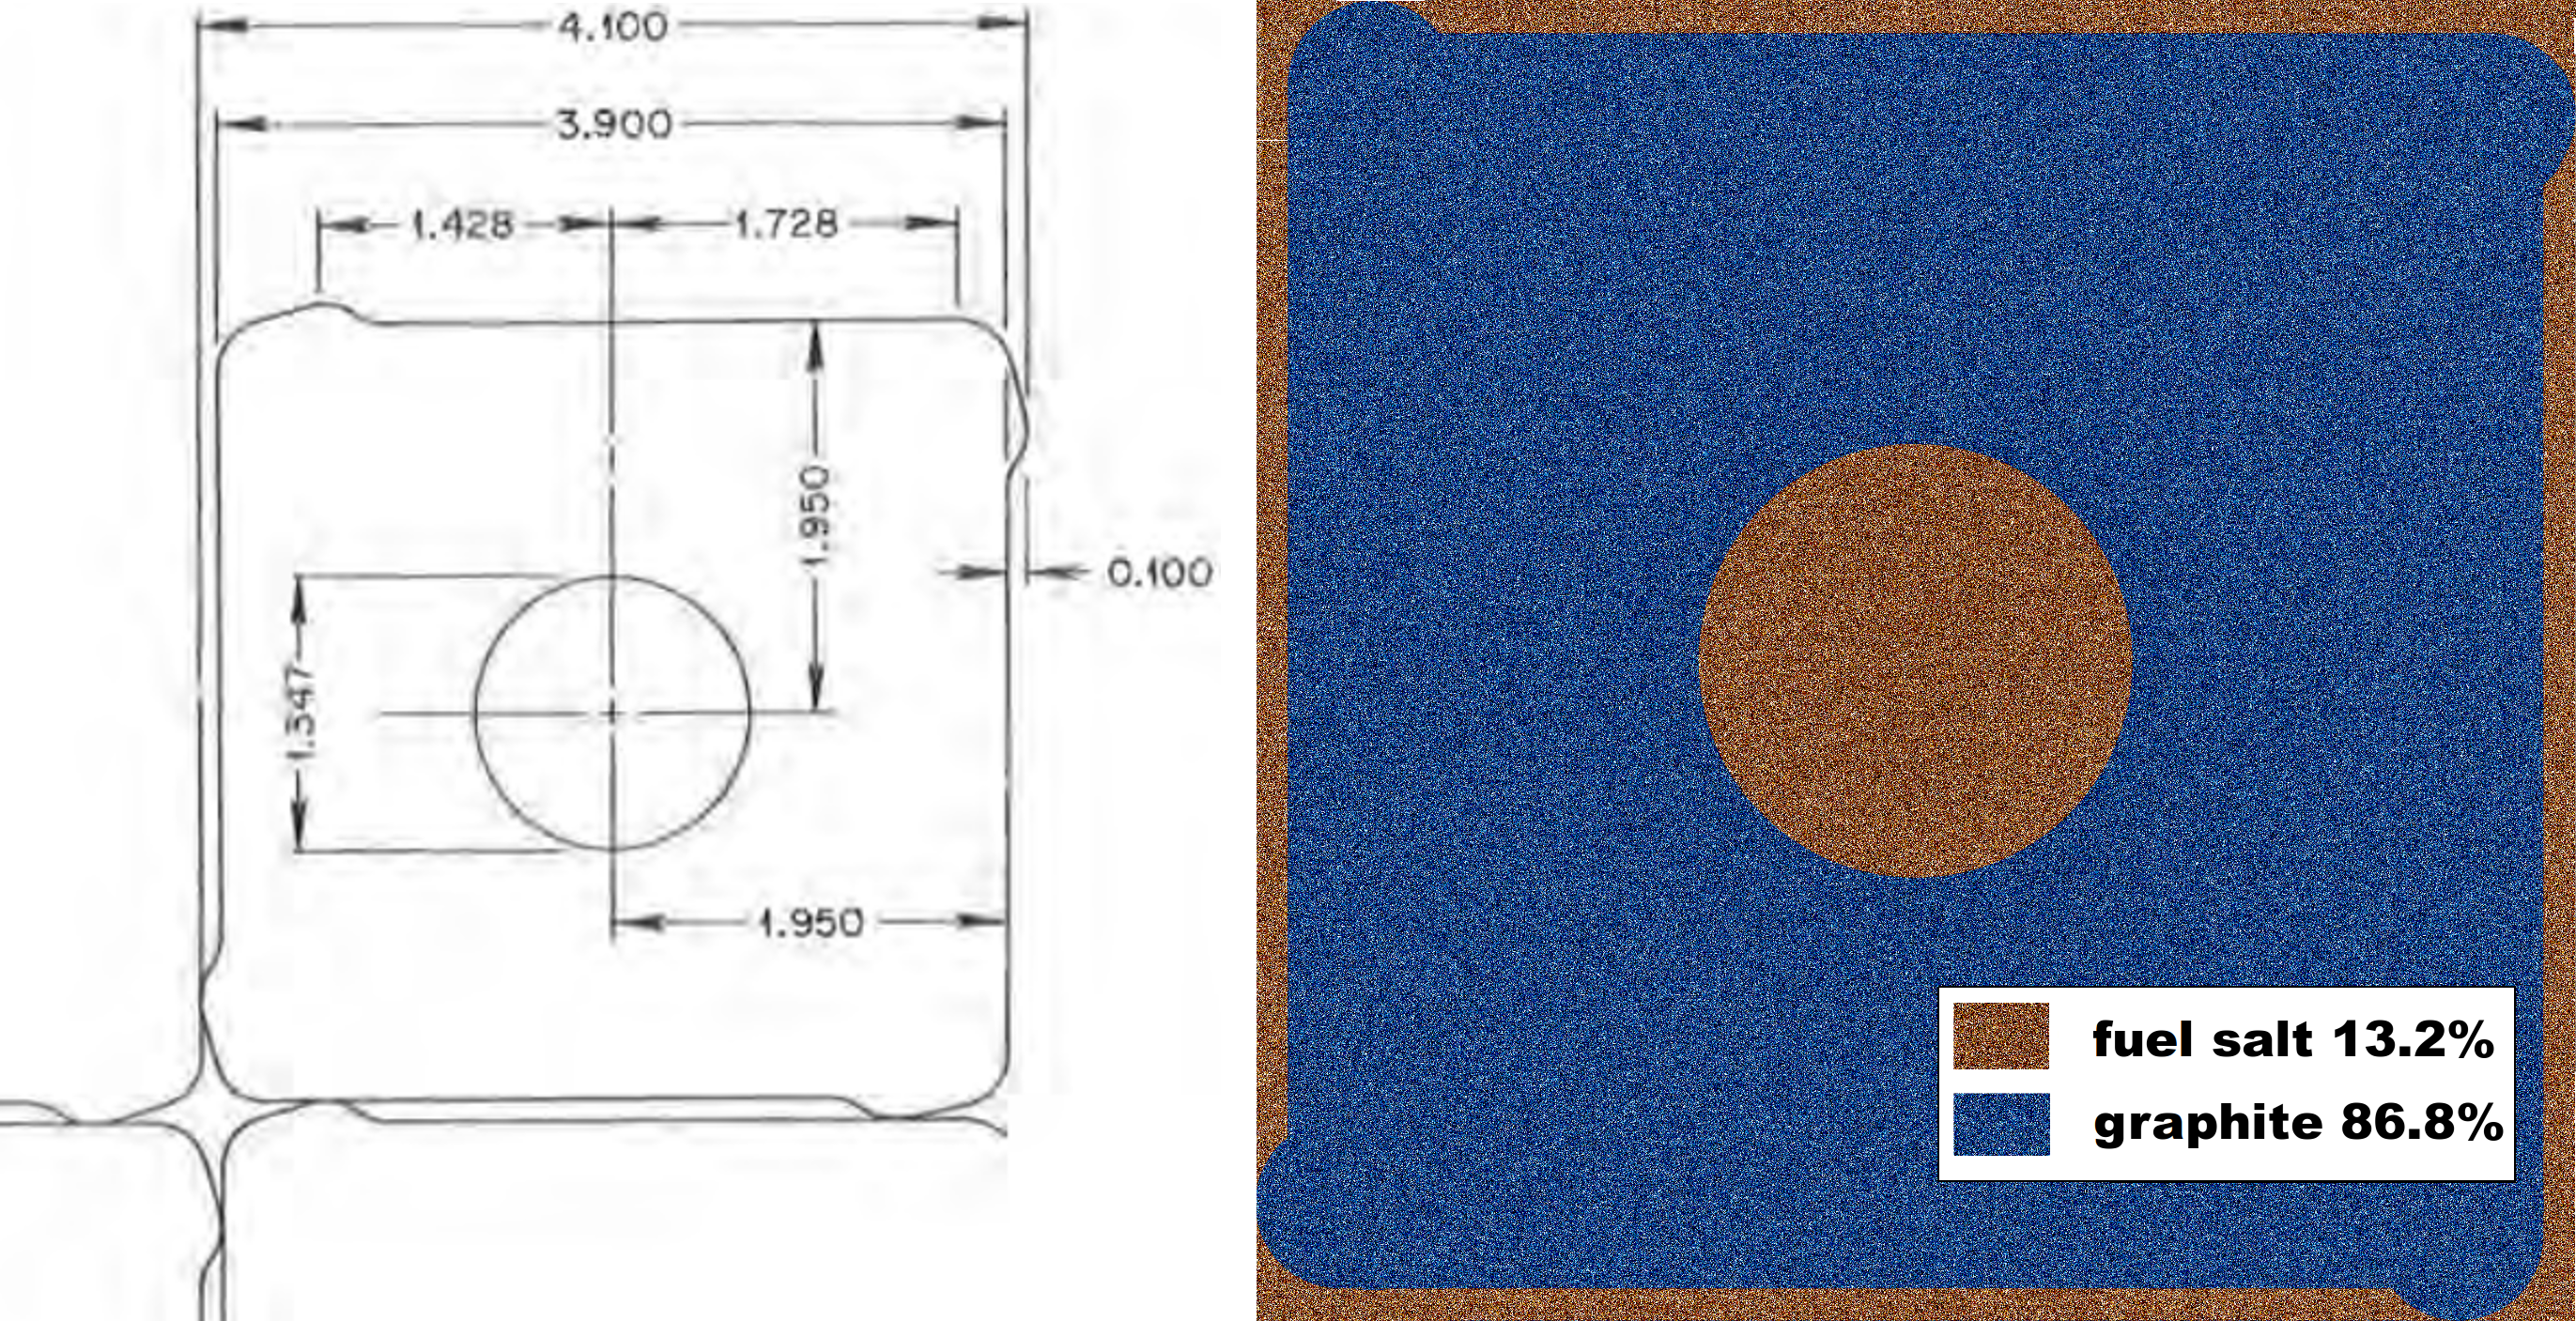
\includegraphics[width=\textwidth]{./images/zone_I_mesh.png}
\vspace{-5mm}
\caption{Molten Salt Breeder Reactor Zone I unit cell geometry from the 
	reference \cite{robertson_conceptual_1971} (left) and Serpent model 
	(right) \cite{rykhlevskii_full-core_2017}.}
\end{figure}
\end{textblock*}

\end{frame}

\begin{frame}
\frametitle{Graphite channels geometry}
\begin{textblock*}{12.5cm}(0.02cm,2.0cm) % {block width} (coords)
\begin{figure}[t]
\includegraphics[width=1.02\textwidth]{./images/detailed_element_xz.png}
\vspace{-5mm}
\caption{Zone I (left) and Zone II (right) reference design 
\cite{robertson_conceptual_1971} and Serpent 
model \cite{rykhlevskii_full-core_2017}.}
\end{figure}
\end{textblock*}

\end{frame}


\begin{frame}
\frametitle{$k_{eff}$ dynamics during 60 years of MSBR operation}
\vspace{-3mm}
\begin{columns}
	\column{4.3cm}
	\begin{block}{Analysis assumptions}
		\fontsize{7}{9}\selectfont
		\begin{itemize}
			\item Full-core Serpent model
			\item Fine time resolution (\textbf{3-day} depletion step)
			\item Slowly extracted elements are removed at the end of the 
			cycle time (e.g., 50 days for RE)
			\item FP removal efficiency \textbf{fixed, ideal}
			\item All $^{233}$Pa removed and \textbf{equal mass of $^{233}$U} 
			fed to the core
			\item Fresh fertile material feed ($^{232}$Th) to maintain salt 
			inventory
		\end{itemize}
	\end{block}
	\vspace{-2mm}
	\begin{block}{Main findings}
	\fontsize{7}{9}\selectfont
	\begin{itemize}
		\item Strong absorbers ($^{234}$U) and fissile materials ($^{235}$U) 
		are built-up
		\item $k_{eff}$ stabilizes after $\approx6$ years
	\end{itemize}  
	\end{block}  	
	
	\column{8cm}
	\begin{figure}[ht!] 
	\begin{overprint}
	\onslide<1>\includegraphics[width=\textwidth]{../dissertation/figures/ch3/keff.png}
	\vspace{-2mm}
	\caption{Effective multiplication factor dynamics for the full-core 
	\gls{MSBR} model \cite{rykhlevskii_modeling_2019}.}
	\onslide<2>\includegraphics[width=\textwidth]{../dissertation/figures/ch3/keff_zoomed.png}
	\vspace{-0.5mm}
	\caption{\textbf{Zoomed} effective multiplication factor dynamics for the 
	full-core \gls{MSBR} model \cite{rykhlevskii_modeling_2019}.}
	\end{overprint}
	\end{figure}
	
\end{columns}
\end{frame}

\begin{frame}
\frametitle{Fuel salt composition evolution in the MSBR}
\begin{textblock*}{12.8cm}(0.03cm,2.6cm) % {block width} (coords)
\begin{columns}
	\column[t]{7cm}
	\vspace{-0.35in}
	\begin{figure}[t]
		\hspace{-5mm}
		\includegraphics[height=0.69\textheight]{../dissertation/figures/ch3/major_isotopes_adens.png}
		\vspace{-0.15in}
		\caption{Normalized number density of major isotopes in the salt
			during 60 years of operation \cite{rykhlevskii_advanced_2018}.}
	\end{figure}
	
	\column[t]{4.5cm}
	\fontsize{7}{9}\selectfont
		\vspace{-3mm}
	\begin{itemize}
		\item<1-> Neutron poisons ($^{234}$U, $^{232}$Pa) accumulation has 
		negative impact on neutronics
		\item<1-> New fissile materials ($^{235}$U, $^{239}$Pu) improved core 
		performance
		\item<1-> $^{233}$U number density almost constant ($\Delta m<0.8\%$) 
		after 16 years of operation
		\item<1-> $^{242}$Th feed rate \textbf{2.4 kg/d is consistent with 
		ORNL results (2.45 kg/d) \cite{betzler_personal_2017}}
		\item<2-> Neutron spectrum \textbf{hardens toward EOL} causing:
		\setbeamerfont*{itemize/enumerate body}{size=\footnotesize}
		\setbeamerfont*{itemize/enumerate subbody}{parent=itemize/enumerate 
		body}
		\setbeamerfont*{itemize/enumerate subsubbody}{parent=itemize/enumerate 
		body}
		\begin{itemize}
			\item<3-> Reduced $^{233}$U breeding
			\item<4->Temperature coefficient ($\alpha_T$) weakened 
			from $-1.64$ to $-1.58pcm/K$
			\item<5->16\% decline in total control rod worth (CRW)
		\end{itemize} 
	\end{itemize}
\end{columns}
\end{textblock*}
\end{frame}


\begin{frame}
\frametitle{Effect of fission products removal}       

\begin{figure}[t] % replace 't' with 'b' to force it to 
	\centering
	\includegraphics[width=0.9\textwidth]{../dissertation/figures/ch3/keff_rem_cases.png}
	 
		\vspace{-3mm}
	\caption{SaltProc-calculated effective multiplication factor for the 
	full-core \gls{MSBR} model with removal of various fission product groups 
	over 10	years of operation \cite{rykhlevskii_modeling_2019}.}
\end{figure}

\end{frame}



\subsection{Lifetime-long depletion: \gls{TAP} MSR}

\begin{frame}
\frametitle{TAP concept design}

\begin{textblock*}{12.7cm}(0.25cm,1.8cm) % {block width} (coords)
	
	\begin{columns}
		\column[t]{5cm}
		\vspace{+5mm}
		%%%%%%%%%%%%%%%%%%%%%%%%%%%%%%%%%%%%%%%%
		\begin{table}[h!]
			\fontsize{7}{9}\selectfont
			\caption{Summary of principal data
				\cite{transatomic_power_corporation_technical_2016}. }
			\vspace{-2mm}
			\begin{tabularx}{\textwidth}{ X  X }
				\hline
				Thermal power				           		& 1250 MW$_{th}  
				$       
				\\ 
				Electric power		                		& 520 MW$_e  
				$ 			 
				\\ 
				Gross thermal efficiency        			& 
				44\%     				 
				\\  
				Outlet temperature							& 
				620$^{\circ}$C         
				\\ 
				Fuel salt components                   & 
				LiF-UF$_4$				 \\  
				Fuel salt composition                  & 72.5-27.5 
				mole\%			 
				\\  
				Startup fissile material                     & 5\% 
				$^{235}$U          	 \\
				Moderator                              & ZrH$_{1.66}$ rods  \\
				Neutron spectrum						& 
				\textbf{thermal/epithermal}                 \\
				Moderator-to-fuel ratio						& 
				\textbf{varies in (0.1099, 1.0)}                 \\
				\hline
			\end{tabularx}
			\label{tab:tap_tab}
		\end{table}
		%%%%%%%%%%%%%%%%%%%%%%%%%%%%%%%%%%%%%%%%%%%%%%%%
		
		\column[t]{6.5cm}
		\hspace{-9mm}
		\begin{figure}      
			\includegraphics[height=0.79\textwidth]{../dissertation/figures/ch4/tap_core_ornl.png}
			\caption{The \gls{TAP} \gls{MSR} schematic core view showing 
				moderator rods configuration at \gls{BOL} 
				\cite{betzler_assessment_2017-1}.}
		\end{figure}
	\end{columns}
	
\end{textblock*}

\end{frame}

\begin{frame}
\frametitle{\gls{TAP} concept full-core high-fidelity Serpent model}
\begin{textblock*}{12.6cm}(0.1cm,1.8cm) % {block width} (coords)
\begin{figure}[htp!] % replace 't' with 'b' to 
	\begin{overprint}
		\onslide<1>\centerline{\includegraphics[height=0.75\textheight]{./images/347_base.png}}
		\onslide<2>\centerline{\includegraphics[height=0.75\textheight]{./images/406.png}}
		\onslide<3>\centerline{\includegraphics[height=0.75\textheight]{./images/576.png}}
		\onslide<4>\centerline{\includegraphics[height=0.75\textheight]{./images/633.png}}
		\onslide<5>\centerline{\includegraphics[height=0.75\textheight]{./images/900.png}}
		\onslide<6>\centerline{\includegraphics[height=0.75\textheight]{./images/1498.png}}
		\onslide<7>\centerline{\includegraphics[height=0.75\textheight]{./images/1668.png}}
	\end{overprint}
	\caption{An $XY$ section of the \gls{TAP} model with various 
	moderator-to-fuel ratio. The violet color represents zirconium hydride, 
	the yellow represents fuel salt \cite{chaube_tap_2019, 
	rykhlevskii_milestone_2019}.}
\end{figure}
\end{textblock*}
\end{frame}



\begin{frame}
\frametitle{$k_{eff}$ dynamics during 23.5 years of TAP operation}
\vspace{-3mm}
\begin{columns}
	\column{4.3cm}
	\begin{block}{Analysis assumptions}
		\fontsize{7}{9}\selectfont
		\begin{itemize}
			\item Quarter-core Serpent model
			\item Fine depletion resolution (\textbf{3-day})
			\item 5\% LEU feed (UF$_4$) to maintain salt inventory
			\item Xe removal efficiency $\epsilon_{Xe}=$\textcolor{green}{
			0.03}, \textcolor{orange}{0.54}, and \textcolor{blue}{0.92} for 
			mass transfer coefficient $K_L=$\textcolor{green}{0.085}, 
			\textcolor{orange}{2.117}, and \textcolor{blue}{8.467}$mm/s$
		\end{itemize}
	\end{block}
	\vspace{-2mm}
	\begin{block}{Main findings}
		\fontsize{7}{9}\selectfont
		\begin{itemize}
			\item $^{235}$U is substituted with $^{239}$Pu
			\item Poisonous $^{234}$U is built-up ($>$1t at EOL)
			\item Total U inventory decreased from 137 to 129t
		\end{itemize}  
	\end{block}  	
	
	\column{8cm}
	\begin{figure}[ht!] 
		\begin{overprint}
			\onslide<1>\includegraphics[width=\textwidth]{../dissertation/figures/ch4/eps/keff.png}
			\onslide<2>\includegraphics[width=\textwidth]{./images/keff_z_1.png}
			\onslide<3>\includegraphics[width=\textwidth]{../dissertation/figures/ch4/eps/keff_zoomed_1.png}
			\vspace{-4mm}
		\end{overprint}
	\caption{SaltProc-calculated effective multiplication factor 
	for the full-core \gls{TAP} concept.}			
	\end{figure}
	
\end{columns}
\end{frame}


\begin{frame}
\frametitle{Neutron energy spectrum}
\begin{textblock*}{12.6cm}(0.1cm,1.7cm) % {block width} (coords)
	\begin{figure}[htp!] % replace 't' with 'b' to 
		\begin{overprint}
\onslide<1>\centerline{\includegraphics[width=0.65\textwidth]{../dissertation/figures/ch4/eps/spectrum.png}}
\onslide<2>\centerline{\includegraphics[width=0.65\textwidth]{./images/tap_sp_z_1.png}}
\onslide<3>\centerline{\includegraphics[width=0.67\textwidth]{../dissertation/figures/ch4/eps/spectrum_th_zoomed.png}}
		\end{overprint}
			\vspace{-3mm}
		\caption{The neutron flux energy spectrum normalized by unit lethargy 
		at the BOL and EOL. The neutron flux uncertainties $\sigma_{\Phi}$ are 
		0.6\% and 0.18\% for the \gls{TAP} reactor and \gls{MSBR}, 
		respectively.}
	\end{figure}
\end{textblock*}
\end{frame}


\begin{frame}
\frametitle{Fuel salt composition evolution during the TAP operation (1/2)}
\begin{textblock*}{12.25cm}(0.25cm,1.8cm) % {block width} (coords)
	\begin{figure}[htp!] % replace 't' with 'b' to 
		\centering
		\includegraphics[width=0.75\textwidth]{../dissertation/figures/ch4/eps/u235.png}
			\vspace{-2mm}
		\caption{SaltProc-calculated mass of $^{235}$U in the fuel salt during 
		25 years of operation
for K$_L$ = 8.4667 mm/s compared with less 
		effective noble gas removal.}
	\end{figure}
\end{textblock*}
\end{frame}

\begin{frame}
\frametitle{Fuel salt composition evolution during the TAP operation (2/2)}
\begin{textblock*}{12.25cm}(0.25cm,1.8cm) % {block width} (coords)
	\begin{figure}[htp!] % replace 't' with 'b' to 
		\centering
		\includegraphics[width=0.77\textwidth]{../dissertation/figures/ch4/eps/pu239.png}
		\vspace{-1mm}
		\caption{SaltProc-calculated mass of $^{239}$Pu in the fuel salt 
		during 25 years of operation for K$_L$ = 8.4667 mm/s compared with 
		less effective noble gas removal.}
	\end{figure}
\end{textblock*}
\end{frame}


\begin{frame}
\frametitle{Impact of xenon poisoning on fuel cycle performance}
\begin{textblock*}{12.4cm}(0.07cm,2.1cm) % {block width} (coords)
	\begin{columns}
		\column[t]{5.5cm}
		\vspace{-5mm}
		\visible<2->
		{\begin{figure}[hbp!] % replace 't' with 'b' to 
			\includegraphics[width=0.94\textwidth]{../dissertation/figures/ch5/tap_vs_pwr_spectrum_2.png}\\
			\vspace{-5mm}
			\hspace{+0.05mm}
			\includegraphics[width=0.94\textwidth]{../dissertation/figures/ch5/i_xe_xs.png}
			\vspace{-3mm}
			\caption{Neutron spectra (upper) and $^{135}$I, $^{135}$Xe caption 
			cross section (lower) \cite{rykhlevskii_impact_2019}.}
		\end{figure}}
		
		\column[t]{6cm}
		\begin{textblock*}{7.3cm}(5.6cm,2.1cm) % {block width} (coords)
		\begin{itemize}
			\itemsep=1em
			\item<1-> \textbf{Less effective} gas removal leads to 
			\textbf{harder} 
			spectrum
			\begin{itemize}
				\itemsep=0.5em
				\item Shorter lifetime due to parasitic absorption
				\item Lower $^{235}$U fission rate
				\item Faster rate of $^{238}$U destruction (-50kg)
				\item Increased breeding of fissile Pu
			\end{itemize}
			
			\item<2-> TAP spectrum \textbf{softens toward EOL}
			\begin{itemize}
				\itemsep=0.5em
				\item Reduced fissile Pu breeding after 11yrs
				\item $\alpha_T$ weakened 
				from $-1.57$ to $-0.26pcm/K$
				\item 12\% CRW degradation
				\item 39\% void coefficient of reactivity ($\alpha_V$) 
				degradation
				\item Lower reactor kinetic parameters ($\beta_{eff}$, 
				$\lambda_{eff}$)
			\end{itemize} 
		\end{itemize}
	
	\visible<3->{\par\small	These observations must be considered during the 
	reactor 
	designing, accident analysis, and safety justification.}
		\end{textblock*}
	
	
	\end{columns}
\end{textblock*}
\end{frame}


\begin{frame}
\frametitle{Uncertainty propagation in depletion calculations (1/2)}
\begin{textblock*}{12.4cm}(0.07cm,1.9cm) % {block width} (coords)
	\begin{columns}
		\column[t]{5.5cm}
		\vspace{-3mm}
		\visible<3->
		{\begin{figure}[hbp!] % replace 't' with 'b' to 
				\includegraphics[width=0.92\textwidth]{../dissertation/figures/uq/serpent_mass_std_u.png}\\
				\vspace{-4.5mm}
				\hspace{+0.3mm}
				\includegraphics[width=0.91\textwidth]{../dissertation/figures/uq/serpent_mass_std_pu.png}
				\vspace{-3.5mm}
				\caption{Stochastic uncertainty in the uranium and plutonium 
				isotopic inventory.}
		\end{figure}}
		
		\column[t]{6cm}
		\begin{textblock*}{7.2cm}(5.5cm,1.7cm) % {block width} (coords)
			\begin{block}<1->{Sources of uncertainty in depletion calculations}
			\begin{itemize}
				\itemsep=0.3em
				\item<2-> Stochastic uncertainty (Monte Carlo)
				\begin{itemize}
					\itemsep=0.5em
					\item Serpent unable to provide statistical error in 
					predicted composition
					\item Depletion with Serpent \textbf{1000 times, only 
					initial random seed changed}
					\item The mean and standard deviation of isotopic 
					concentration calculated from 1000 samples
				\end{itemize}
				
			\end{itemize}
			\end{block}
			
		\end{textblock*}

	\end{columns}
\end{textblock*}
\end{frame}

\begin{frame}
\frametitle{Uncertainty propagation in depletion calculations (2/2)}
\begin{textblock*}{12.4cm}(0.07cm,1.9cm) % {block width} (coords)
	\begin{columns}
		\column[t]{5.5cm}
		\vspace{-4mm}
		\visible<2->
		{\begin{figure}[hbp!] % replace 't' with 'b' to 
				\includegraphics[width=0.9\textwidth]{../dissertation/figures/uq/scale_mass_std_u.png}\\
				\vspace{-4.5mm}
				\hspace{+0.1mm}
				\includegraphics[width=0.9\textwidth]{../dissertation/figures/uq/scale_mass_std_pu.png}
				\vspace{-3.5mm}
				\caption{Nuclear data-related uncertainty \newline in U and Pu 
				isotopic 
				inventory.}
		\end{figure}}
		
		\column[t]{6cm}
		\begin{textblock*}{7.2cm}(5.5cm,1.7cm) % {block width} (coords)
			\begin{block}<1->{Sources of uncertainty in depletion calculations}
				\begin{itemize}
					\itemsep=0.3em
					\item<3> Stochastic uncertainty (Monte Carlo)
					\begin{itemize}
						\itemsep=0.5em
						\item Serpent unable to provide statistical error in 
						predicted composition
						\item Depletion with Serpent \textbf{1000 times, only 
							initial random seed changed}
						\item The mean and standard deviation of isotopic 
						concentration calculated from 1000 samples
					\end{itemize}
					
					\item<1-> Uncertainty in the nuclear data
					\begin{itemize}
						\itemsep=0.5em
						\item Nuclear data covariance propagated via 
						depletion calculations using SCALE Sampler
						\item Simple unit-cell model (NEWT)
						\item Collection of random nuclear data files 
						generated from a multivariate normal distribution and 
						covariances
						\item 800 random samples
					\end{itemize} 
				\end{itemize}
			\end{block}
			\visible<3->{\small \textbf{Takeaway:} Nuclear-data related 
			uncertainty $\times100$ 
			greater that 
			stochastic}
				
		\end{textblock*}
		
	\end{columns}
\end{textblock*}
\end{frame}
\subsection{Short-term depletion: TAP MSR}


\begin{frame}
\frametitle{Why is load following a game changer?}
\begin{textblock*}{12.1cm}(0.3cm,1.65cm) % {block width} (coords)
	\begin{figure}[t]
		\includegraphics[width=0.65\textwidth]{./images/ne_one_day_price.png}
		\vspace{-2mm}
		\caption{ISO New England hourly electricity price; Nov 3, 2019 
			from 00:00AM to 11:00PM (Source: https://www.iso-ne.com/).}
	\end{figure}  
	\vspace{-4mm}
	
	\visible<2->{\begin{block}{Physical constrains limiting power 
	variations	in 
				Light-Water	Reactors \cite{lokhov_technical_2011}:}
			\begin{itemize}
				\item thermal strain and stress to fuel materials
				\item fuel burnup (insufficient excess reactivity at the 
				EOC)}
			\item<3-> \textbf{$^{135}Xe$ poisoning (iodine pit)}
		\end{itemize}
	\end{block}
\end{textblock*}
\end{frame}


\begin{frame}
\frametitle{What is $^{135}$Xe poisoning? \cite{nuclear_power_production_2020}}
\animategraphics[loop,controls,width=1.07\linewidth]{0.5}{./images/anime/xe_pois-}{0}{11}
\end{frame}


\begin{frame}
\frametitle{Postulated worst-case load-following scenario}
\vspace{-6mm}
\begin{columns}
	\column[t]{5.5cm}
	\begin{figure}[t]
		\includegraphics[width=\linewidth]{./images/power_load_curve.png}
		\vspace{-6mm}
		\caption{Postulated load-following power transient.}
	\end{figure}
	
	\column[t]{6.3cm}
	\begin{block}{Postulated load-following transient}
		\begin{enumerate}             
			\item operation on 100\% power	level for \textbf{$t_{eq}$} to 
			reach $^{135}$Xe/$^{135}$I equilibrium
			\item instantaneous power drop from 100 to 0\%
			\item shutdown for \textbf{$t^{max}_{X}$} to reach the 
			$^{135}$Xe peak
			\item restart instantly from 0 to 100\%, and then operation on 
			100\% for a few hours
		\end{enumerate}
			\vspace{-8mm}
	\end{block}
		\begin{align}\label{eq:time-xe-max}
		t^{max}_{X} &= \frac{1}{\lambda_X-\lambda_I}
		log\left(\frac{\lambda_X(\lambda_I[X_0+I_0]-\lambda_XX_0)}{\lambda_I^2 
		I_0}\right) \nonumber
		\end{align}
	\begin{block}{Simplifying assumptions}
		\begin{itemize}
			\item All control rods are fully withdrawn
			\item Power adjusted by changing normalization in Serpent 2
			\item 15-min depletion step
		\end{itemize}
		
	\end{block}
\end{columns}
\end{frame}

\begin{frame}
\frametitle{TAP load-following simulation without gas removal outcomes}
\begin{textblock*}{12.5cm}(0.1cm,2.1cm) % {block width} (coords)
\begin{columns}
	\column[t]{6.3cm}
	\begin{figure}[t]
		\begin{overprint}
	\onslide<2>\includegraphics[width=1.11\linewidth]{../dissertation/figures/ch5/keff_kl_1_eol_eoc_15min.png}
		\vspace{-6mm}
	\caption{$k_{eff}$ dynamics during 2.75-hour shutdown (\textbf{10 days 
		before EOL}, \textbf{no gas removal}). $\sigma\pm7$ $pcm$ is shaded.}
	\onslide<3-4>\includegraphics[width=1.11\linewidth]{../dissertation/figures/ch5/xe_i_kl_1_eol_eoc_15min.png}
		\vspace{-6mm}
	\caption{Number density of $^{135}$Xe and $^{135}$I during anticipated 
	transient (\textbf{10 days before EOL}, \textbf{no gas removal}).}
		\end{overprint}
	\end{figure}
	
	\column[t]{5.5cm}
	\begin{textblock*}{6cm}(6.65cm,2.1cm) % {block width} (coords)
		\fontsize{7}{9}\selectfont
		\begin{itemize}
		\item<1-> Negligible xenon poisoning at BOL
	\setbeamerfont*{itemize/enumerate body}{size=\footnotesize}
	\setbeamerfont*{itemize/enumerate subbody}{parent=itemize/enumerate 
	body}
	\setbeamerfont*{itemize/enumerate subsubbody}{parent=itemize/enumerate 
	body}			
			\begin{itemize}
				\item $\rho_X\approx-10\pm7$ $pcm$
				\item $^{135}$Xe concentration change $+0.33$\%
				\item $N_{^{135}I}/N_{^{135}Xe}<0.8$ due to hard spectrum
			\end{itemize} 
			\item<2-> Weak xenon poisoning at EOL (10d before shutdown, all 
			moderator rods are inserted)
	\setbeamerfont*{itemize/enumerate body}{size=\footnotesize}
	\setbeamerfont*{itemize/enumerate subbody}{parent=itemize/enumerate 
		body}
	\setbeamerfont*{itemize/enumerate subsubbody}{parent=itemize/enumerate 
		body}			
			\begin{itemize}
				\item $\rho_X\approx-70\pm7$ $pcm$
				\item<3-> $^{135}$Xe concentration change $+4$\%
				\item<3-> $N_{^{135}I}/N_{^{135}Xe}\approx1.0$
			\end{itemize}
		\end{itemize}
				\vspace{+5mm}
		\begin{block}<4->{\qquad Main takeaways}
			\begin{itemize}
				\item TAP \textbf{can load-follow} throughout whole
			lifetime \textbf{without significant $^{135}$Xe poisoning}
				\item Noble gas removal \textbf{unnecessary for load-following}
				\item Main reason - \textbf{relatively fast neutron spectrum} 
				of TAP MSR
			\end{itemize}
		
	\end{block}
	\end{textblock*}
\end{columns}
\end{textblock*}
\end{frame}



\begin{frame}
\frametitle{Safety parameters evolution during load-following (EOL)}
\begin{textblock*}{12.5cm}(0.1cm,2.1cm) % {block width} (coords)
	\begin{columns}
		\column[t]{6.3cm}
		\begin{figure}[t]
			\begin{overprint}
	\onslide<1>\includegraphics[width=1.15\linewidth]{../dissertation/figures/ch5/saf_par/tc_evo.png}
	\vspace{-6mm}
	\caption{Temperature feedback coefficients as a function of time during 
	the transient. 
	Uncertainty $\pm\sigma$ is shaded.}
	\onslide<2>\includegraphics[width=1.15\linewidth]{../dissertation/figures/ch5/saf_par/void_evo.png}
	\vspace{-6mm}
	\caption{Void coefficient of reactivity ($\alpha_V$) as a function of time 
	during the transient.}
	\onslide<3->\includegraphics[width=1.15\linewidth]{../dissertation/figures/ch5/saf_par/crw_evo.png}
	\vspace{-6mm}
	\caption{Total control rod worth as a function of time during the 
	transient.}
			\end{overprint}
		\end{figure}
		
		\column[t]{5.5cm}
		\begin{textblock*}{5.9cm}(6.9cm,2.6cm) % {block width} (coords)
			\begin{itemize}
				\itemsep=0.8em
				\item<1-> Fuel temperature coefficient ($\alpha_{T,F}$) 
				weakened during first 3 hours when $^{135}$Xe concentration 
				peaked causing the spectrum hardening
				\item<2-> $\alpha_V$ fluctuates in stochastic uncertainty 
				range $\sigma_{\alpha_V}\pm4$ $pcm/$\%
				\item<3-> CRW worsened right after shutdown but then quickly 
				recovered due to quick $^{135}$Xe removal
				\item<4-> TAP reactor maintains safety margins during the 
				load-following transient
			\end{itemize}
				
		\end{textblock*}
	\end{columns}
\end{textblock*}
\end{frame}


\subsection{Short-term depletion: MSBR}

\begin{frame}
\frametitle{Xenon poisoning effect during MSBR load-following}
\vspace{-7mm}
\begin{columns}
	\column[t]{7cm}
	\visible<2->{
	\begin{figure}[t]
	\centering
$\begin{array}{r}
\includegraphics[width=0.707\textwidth]{../dissertation/figures/ch6/kl1_rho.png}\vspace{-5mm}\\
\includegraphics[width=0.69\textwidth]{../dissertation/figures/ch6/kl25_rho.png}\vspace{-5mm}\\
\includegraphics[width=0.69\textwidth]{../dissertation/figures/ch6/kl100_rho.png}
\end{array}$
\vspace{-4mm}
\caption{$\rho(t)$ during the transient ($\pm\sigma_{\rho}=10$$pcm$).}
	\end{figure}}
	
	\column[t]{5.5cm}
	\begin{textblock*}{6.1cm}(6.3cm,2.1cm) % {block width} (coords)
	\begin{block}<1->{Analysis assumptions}
				\fontsize{7}{9}\selectfont
		\begin{enumerate}             
			\item Load profile similar to TAP reactor
			\item $t^{max}_X\approx7.5h$
			\item 30-min depletion step
			\item Low, medium, and high gas removal efficiency
		\end{enumerate}
		\vspace{-4mm}
	\end{block}

	\begin{block}<2->{Key takeaways}
				\fontsize{7}{9}\selectfont
		\begin{itemize}
			\item MSBR \textbf{cannot load-follow without gas removal:} 
			$\Delta\rho=-1490pcm$
			\item Xenon poisoning is \textbf{milder toward EOL} due to 
			spectrum \textbf{hardening}
			\item Huge \textbf{positive reactivity insertion} for medium 
			and high removal efficiency
			\item Even removal of \textbf{53.6\%} of Xe significantly 
			reduced the effect of poisoning: \textbf{-161$\pm10pcm$}
			\item More effective removal (\textbf{91.5\%}) gave similar 
			improvement: \textbf{-189$\pm10pcm$}
		\end{itemize}
		
	\end{block}
\end{textblock*}
\end{columns}
\end{frame}

\begin{frame}
\frametitle{Safety parameters evolution during load-following}
\begin{textblock*}{12.5cm}(0.4cm,1.55cm) % {block width} (coords)
	\begin{columns}
		\column[t]{6.3cm}
		\begin{figure}[t]
			\begin{overprint}
				\onslide<1>\includegraphics[width=0.87\linewidth]{./images/msbr_tc_evo.png}
				\vspace{-2mm}
				\caption{Temperature coefficients dynamics during the 
				transient.}
				\onslide<2>\includegraphics[width=0.87\linewidth]{./images/msbr_void_evo.png}
				\vspace{-2mm}
				\caption{Void coefficient of reactivity ($\alpha_V$) dynamics
					during the transient.}
				\onslide<3->\includegraphics[width=0.87\linewidth]{./images/msbr_crw_evo.png}
				\vspace{-2mm}
				\caption{Total control rod worth dynamics during 
				the transient.}
			\end{overprint}
		\end{figure}
		
		\column[t]{6cm}
		\begin{textblock*}{6.7cm}(6cm,2.6cm) % {block width} (coords)
			\begin{itemize}
				\itemsep=0.8em
				\item<1-> $\alpha_{T,ISO}$ worsens slightly as $^{135}$Xe 
				concentration spiked and then improves quickly
				\item<2-> $\alpha_V$ demonstrates similar behavior
				\item<3-> CRW worsened after shutdown but then quickly 
				recovered due to quick $^{135}$Xe removal
				\item<4-> Total control rod worth is insufficient to shut down 
				the reactor at any time during transient
			\end{itemize}
			
		\end{textblock*}
	\end{columns}
\end{textblock*}
\end{frame}


\begin{frame}
\frametitle{Neutron energy spectrum MSBR vs TAP}
\begin{textblock*}{12.6cm}(0.1cm,1.6cm) % {block width} (coords)
	\begin{figure}[htp!] % replace 't' with 'b' to 
		\centerline{\includegraphics[width=0.73\textwidth]{../dissertation/figures/ch6/msbr_vs_tap_spectrum.png}}
		\vspace{-3mm}
		\caption{The neutron flux energy spectrum normalized by unit lethargy 
		for 
			MSBR and TAP at BOL and EOL. }
	\end{figure}
\end{textblock*}
\end{frame}
\section{Conclusions}
\begin{frame}
\frametitle{Conclusions}
\begin{textblock*}{12cm}(0.4cm,1.8cm) % {block width} (coords)
	\begin{itemize}
		\itemsep1em
		\item Relevance
		\begin{itemize}
			\itemsep0.5em
			\item MSR fuel salt processing system modeling is typically based 
			on \textbf{many assumptions and estimations}
			\item \textbf{Realistic, multi-component} salt 
			processing system modeling capabilities are required for advanced 
			\gls{MSR} analysis
		\end{itemize} 
		\item The current work \textbf{contributes} to the nuclear engineering 
		community by providing \textbf{open-source tool for fuel depletion 
		analysis in liquid-fueled nuclear systems}
			\begin{itemize}
			\itemsep0.5em
			\item Source code available at 
			\url{https://github.com/arfc/saltproc/}
			\end{itemize}
		\item We demonstrated tool capabilities for \textbf{two MSRs at 
		various time scales}
		\begin{itemize}
			\itemsep0.5em
			\item Lifetime-long depletion with \textbf{ideal/realistic removal 
			efficiency} and \textbf{variable geometry}
			\item Short-term load-following transient simulation to 
			evaluate \textbf{effect of online gas removal on xenon poisoning}
		\end{itemize}
		\item We analyzed safety parameters evolution during long- 
		and short-term cases and confirmed that the \textbf{critical safety 
		margins are maintained}
		\item Simplified UQ analysis shown that \textbf{stochastic error} in 
		predicted composition is \textbf{negligible} comparing with 
		\textbf{nuclear-data related error}
	\end{itemize}
\end{textblock*}
\end{frame}

\begin{frame}
\frametitle{Future work}
\begin{textblock*}{12cm}(0.4cm,2.2cm) % {block width} (coords)
	\begin{block}{Possible future research effort}
		\begin{enumerate}
			\itemsep1em
			\item Extend validation portfolio with other MSR designs (e.g., 
			Single-fluid Double-zone Thorium Molten Salt Reactor which we 
			recently modeled using Serpent 2 \cite{ASHRAF2019107115})
			\item Extend load-following simulations of realistic load 
			profiles
			\item Perform in-depth sensitivity analysis by varying gas removal 
			efficiency to bound gas removal system design
			\item Develop a fuel processing system model for SaltProc
			for a \textbf{various commercial molten salt reactor concepts}
			\begin{itemize}
				\itemsep0.5em
				\item Integral Small Modular Reactor from Terrestrial Energy
				\item Small Modular Molten Salt Reactor from ThorCon
				\item Liquid Fluoride Thorium Reactor from Flibe
energy 
			\end{itemize}
			\item Estimate long-term financial benefits from noble gas removal
		\end{enumerate}
	\end{block}
\end{textblock*}
\end{frame}



\begin{frame}
	\frametitle{Questions?}
\end{frame}
%%--------------------------------%%
%%--------------------------------%%
\appendix
\begin{frame}[allowframebreaks]
  \frametitle{References}
  \bibliographystyle{unsrt}
  {\footnotesize \bibliography{../dissertation/thesisrefs} }

\end{frame}

%%--------------------------------%%
%%---BACKUP SLIDES----------------%%
\begin{frame}
\frametitle{SaltProc architecture}
\vspace{-2mm}
\begin{figure}[ht!] % replace 't' with 'b' to \centering
\includegraphics[width=0.84\textwidth]{../dissertation/figures/ch2/saltproc_class_diagram.png}
	\caption{SaltProc v1.0 python package class diagram in UML notation 
		with examples of object instances.}
\end{figure}
\end{frame}	


\begin{frame}
\frametitle{Extraction rate for various reactors}
\begin{textblock*}{12.5cm}(0.5cm,1.6cm) % {block width} (coords)
%%%%%%%%%%%%%%%%%%%%%%%%%%%%%%%%%%%%%%%%
\begin{table}[htbp!]
\fontsize{6}{9}\selectfont
\centering
\caption{The effective cycle times and rates for fission products 
removal \cite{robertson_conceptual_1971, betzler_implementation_2017}.}
\vspace{-2mm}
\begin{tabular}{p{0.14\textwidth} p{0.3\textwidth} p{0.11\textwidth} 
p{0.11\textwidth}}
\hline 
\textbf{Processing group} & \qquad\qquad\qquad \textbf{Nuclides} & 
\textbf{Removal Rate (s$^{-1}$)} & \textbf{Cycle time (at full 
power)} 
\\ \hline 
\multicolumn{3}{c}{\textit{Elements removed in \gls{MSBR} and 
adopted for the \gls{TAP}} 
\cite{robertson_conceptual_1971}} \\
Noble gases & Xe, Kr								  & 5.00E-2 & 
20 
sec \\
Noble metals & Se, Nb, Mo, Tc, Ru, Rh, Pd, Ag, Sb, Te & 5.00E-2 & 
20 
sec \\
Seminoble metals & Zr, Cd, In, Sn	  				  & 5.79E-8 & 
200 
days\\
Volatile fluorides & Br, I 							  & 1.93E-7 & 
60 
days\\
Rare earths & Y, La, Ce, Pr, Nd, Pm, Sm, Gd           & 2.31E-7 & 
50 
days\\
\qquad & Eu & 2.32E-8 & 500 days \\
Discard & Rb, Sr, Cs, Ba & 3.37E-9 & 3435 days \\
\hline
\multicolumn{3}{c}{\textit{Additional elements removed in 
\gls{TAP}} 
\cite{betzler_implementation_2017, 
transatomic_power_corporation_neutronics_2016}} \\
Noble gases & H								  	& 5.00E-2 & 20 
sec    \\
Noble metals & Ti, V, Cr, Cu						& 3.37E-9 & 
3435 
days \\
Seminoble metals & Mn, Fe, Co, Ni, Zn, Ga, Ge, As   & 3.37E-9 & 
3435 
days \\
Rare earths & Sc									& 3.37E-9 & 
3435 
days \\
Discard & Ca										& 3.37E-9 & 
3435 
days \\
\hline
\multicolumn{3}{c}{\textit{Additional elements removed in 
\gls{MSBR}} 
\cite{robertson_conceptual_1971}} \\
Protactinium & Pa  	& 3.86E-6 & 3 days    \\
\hline
\end{tabular}
\label{tab:reprocessing_list}
\end{table}
\begin{itemize}
\item \textbf{Noble gas} removal efficiency: variable, defined using 
mathematical model
\item Other FP removal efficiency: fixed and based on 
Table~\ref{tab:reprocessing_list}
\end{itemize}
\end{textblock*}
\end{frame}



\end{document}



